\chapter{Related Work}
\label{ch:relatedwork_report}

\section{Current Research in Using Multiple Analysis Tools}

In the current research, we could see the usage of multiple tools in the software industry, where each tool is different in computation approaches. One could be standard run on nightly builds, for example, with Checkmarx \cite{checkmarx} tool or could be following incremental analysis, which means only testing the changed version of code instead of running analysis on complete codebase. The reasons for using multiple tools could be as each tool is capable of detecting bugs with different coverage, \cite{bessey2010few} \cite{delaitre2015evaluating} it could help in finding more bugs easily which are not found by tool but the other. \cite{plakosh2014improving} There is also research \cite{flynn2018prioritizing} going in the direction of using multiple static analysis tools in order to prioritise the bug warning alerts. There is a paper \cite{meng2008approach} published in 2008 which uses results of three different static analysis tools for a programming language, Java and merges them in order to show warnings to the developer. \\ \\

Caitlin et al. and team developed a framework called Tricorder \cite{tricorder} which mentions about using multiple tools where each tool covers separate bug coverage. The results are displayed during the code review and published by a bot called ReviewBot. They evaluated with a summative approach using click rates by the user, which shows which tool is better in comparison to others. Tricorder is closed source for Google infrastructure, and so this is specific for Google developers. Later, emerges a new tool which is similar to Tricorder with the philosophy behind it, such as workflow integration, data-driven usability improvements, empower users to contribute were transformed into development of Shipshape \cite{shipshape} which is an open-source static program analysis platform. It allows custom analysers to plug in through a standard interface. This tool commonly runs as a command-line interface. It has a different architecture to support the needs of open-source projects. However, the Tricorder influences heavily on its API and design. The drawbacks of this tool being it is heavily dependent on docker and not much workflow integration points with no feedback collection. Google developers archived this project because of the lack of active development. Recently, a new tool from Google called Tricium, which is also open source and more focussed for Chromium development workflow, i.e., Chrome infrastructure with philosophy or ideas from Tricorder. Tricium supports robot comments like Tricorder does, which is unlike with Shipshape having only command-line interface. \\ \\

Cristina et al. and team developed a framework called Parfait \cite{parfait} using multiple tools which address the issues with scalability and precision. For scalability, it checks the easy and expensive analysis for each bug type and for precision it tracks each bug whether it is real, potential or not. \\ \\

Although we have seen the current research trends and their direction, the usability aspect is not addressed so far in the context of using multiple tools. There are no research papers found addressing the usability issue with multiple tools in a single interface. The multiplicity of tools used for a single project and that too with different computation capabilities brings a new challenge. One tool could produce results in no time and others could take more time in comparison. This indifference could lead to a situation of breaking the usability of the user interface. On that challenge, this thesis aims to address such a scenario with a problem statement as “How to integrate the results of multiple static analysis tools in a unified user interface?”. \\ \\

The thesis work begins by brainstorming on the problem statement. As a result, different research questions are brought up. Out of which, we selected three primary questions concerning available sources, scope and limitations of thesis time frame. \\ \\


\section{What Current Tools do?}

Let us now examine each research question and see what the current tools behave like in similar scenario. \\ \\

\textbf{1. How to display the results of the same codebase from different analysis tools?} \\

This question needs to address the scalability aspect of displaying results as usage of multiple tools results in redundancy and a high number of warnings with more coverage. The following \autoref{fig:findbugs-results} shows how a FindBugs \cite{findbugs} static analysis tool shows results for a project \cite{findbugs-example}. This kind of display could be the same with other tool, and so when we use multiple tools, there is a need for a better user interface. \\ \\

\begin{figure}[hbt!]
	\centering
	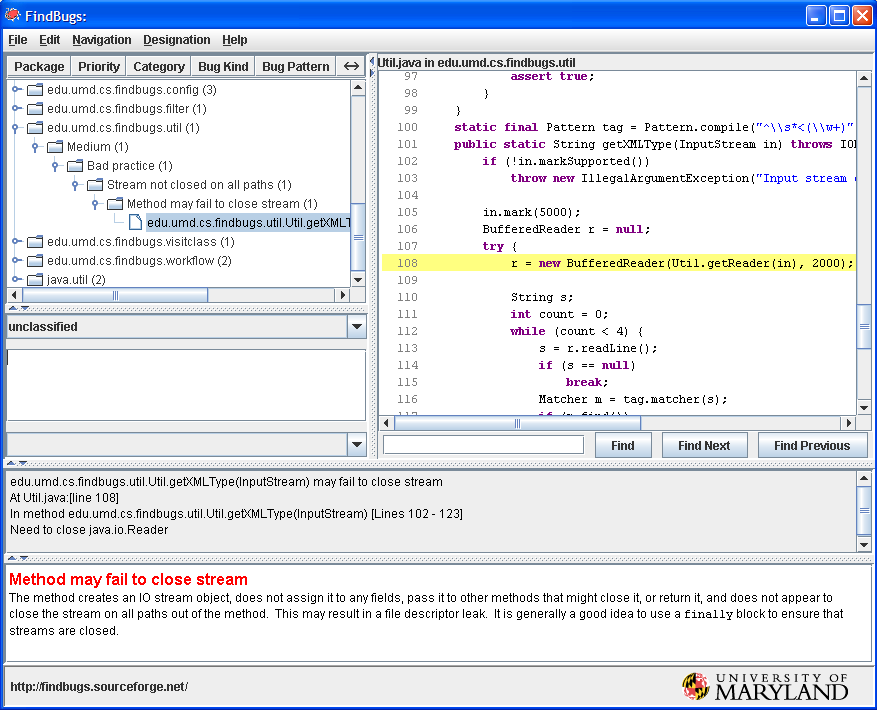
\includegraphics[width=\linewidth]{figures/findbugs-results}
	\caption{A preview of FindBugs scan results.}
	\label{fig:findbugs-results}
\end{figure}

\clearpage

The Tricorder shows the results with multiple tools, as seen in the following \autoref{fig:tricorder-results}, where two findings each from different tool. \\ \\

\begin{figure}[hbt!]
	\centering
	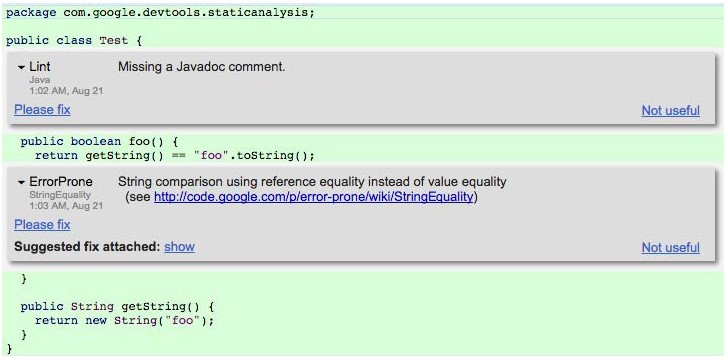
\includegraphics[width=\linewidth]{figures/Tricorder}
	\caption{A preview of Tricorder scan results. \cite{tricorder}}
	\label{fig:tricorder-results}
\end{figure}

\textbf{2. What feedback works to know that the bug fixing is on-going?} \\

This question needs to address the scenario where one tool could give an instant update on the bug fixing process, and others might take more time to analyse and report the update on it. In the design aspect, especially the User Interface needs to be adaptive \cite{NB18} enough as static analysis tools sometimes take a long time to stop, and there is no intuitive feedback provided. Also, One exciting aspect of Johnson et al. \cite{JSMB13} study is about the importance of feedback from tools without disrupting the developer workflow. Traditionally, the project files are added to FindBugs \cite{findbugs} tool as seen in the \autoref{fig:findbugs-scan} in order to start the scanning. Then the user has to wait for some minutes to see the results. There was no feedback in the process of scanning. \\ \\

\begin{figure}[hbt!]
	\centering
	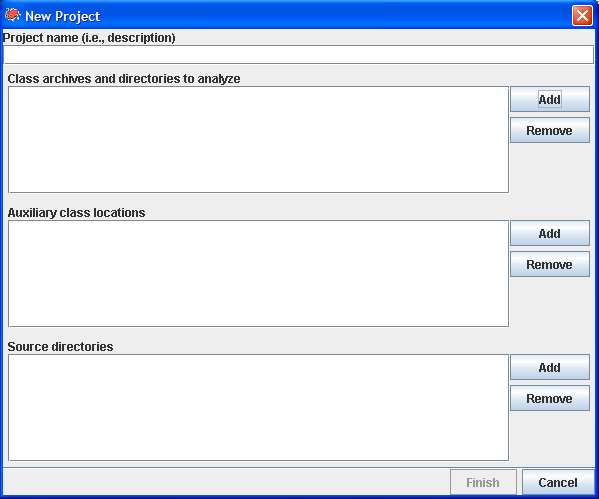
\includegraphics[width=\linewidth]{figures/findbugs-scan}
	\caption{A preview of initiating FindBugs to scan a project. \cite{findbugs}}
	\label{fig:findbugs-scan}
\end{figure}

Back in the history of Computer Science, there is an observation made when the user interface is non-responsive, the user shuts down the system. After that, comes to the implementation of user interface called Ghost screen by Colleran et al. \cite{colleran} who patented the method which manages application programs with non-responsive user interfaces in the year 2005. About the response times, NN Group \cite{nn} states that if the execution of a particular task takes 0.1 up to 1 second, then there is no need for feedback, show the result. If it takes 10 seconds, there should be feedback, and if it is variable every time, then per cent bar \cite{Borman} is essential. However, sometimes, it could be overkill to use as it causes stress to the user by the principle of display inertia. If the time taken by a task is unknown, then there has to be feedback like a spinning ball. If in an example of a task being to scan databases, then it has to report user about what tool scans the database currently. Overall, there has to be feedback stating that the system is working, if not indicating what is doing. This time indifference motivates to know how responsiveness in terms of usability is vital to consider in the development of modern tools. Further, we need to address this in the context of using multiple tools. \\ \\

\textbf{3. How to carry traceability of bug fixing?} \\

In the scenario, where the user has picked a bug to fix and worked on it and later he submitted for analysis. Then the bug could either get fixed or new bugs could have been introduced or different bugs got resolved by fixing the one bug. All these might have taken place, and this is uncertain. Thereby it would be better to have traceability in order to monitor the changes happening in the context of bugs or somehow safeguard the code repository from future bugs. \\ \\

As per the related work in research, \cite{heinemann2014teamscale} a tool named ‘Teamscale’ \cite{teamscale} shows the influence on the quality status for each change in code backed by version control commits. For a change, it shows how many newly added quality problems or the ones removed. Following \autoref{fig:teamscale} illustrates further. \\ \\

\begin{figure}[hbt!]
	\centering
	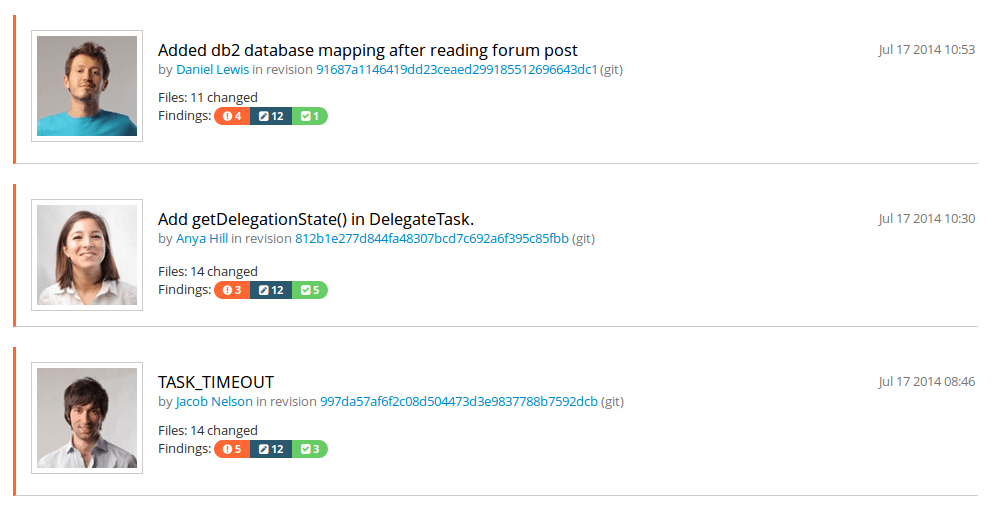
\includegraphics[width=\linewidth]{figures/teamscale}
	\caption{A Teamscale feature of showing quality status with code changes. \cite{teamscale}}
	\label{fig:teamscale}
\end{figure}

\let\cleardoublepage\clearpage
